\section{Current Modern Models}
\begin{wrapfigure}{l}{0.4\textwidth}
\centering
    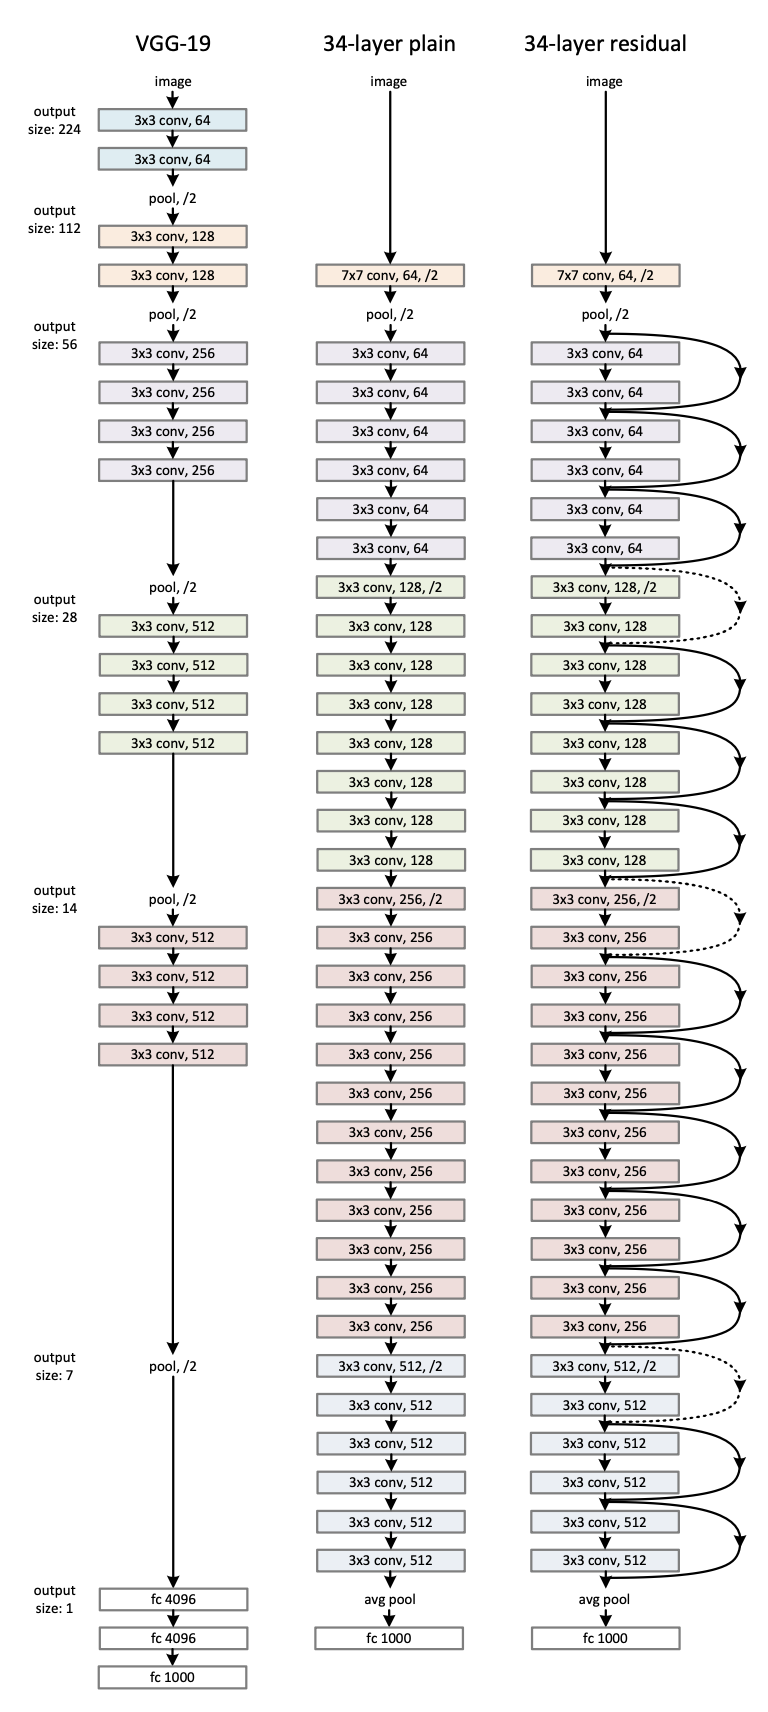
\includegraphics[width=0.35\textwidth]{ResNet50Graph.png}
    \caption{Block Diagram of VGG-19, Precursor to ResNet, and ResNet-34 \cite{ResNet50:He}}
    \label{fig:ResNet50Graph}
\end{wrapfigure}
In the previous section we observed a scaling property of model size as it relates to number dimensions of the data, $O(n^2)$. Also the model would scale as $O(k)$ for $k$ features Many modern problems operate on images data, which abstractly is very high dimensional data. A model would take an image as an input and returns the feature of that image as a classification. That is, the model would return if an image contains a boat or a cat. Even analyzing sets of small images will cause traditional models to be uncomputable. For example a small preview image may be 150 by 150 pixels in 3 channels which gives 67.5k dimensions. A classic model would need about 4.5B parameters. Aside from this many parameters pushing the limits of computing machines, there are classic abstract reasons parameterizing a distribution of this size is intractable and would only be used in the most exotic circumstances. This is where modern Machine Learning (ML) enters the picture. It is beyond the scope of this document to heuristically explore the development of ML from first principles in a way we did with the Iris dataset. Instead we explore one of the more recent and successful models developed, ResNet50 \cite{ResNet50:He}. ResNet50 has about 23M trainable parameters which is 3 orders of magnitude less than the modest estimate above for a classic approach. Just as the Gaussians in the  GMM had a distinct formula, so does ResNet50. It was intentional that the formula for the Gaussian, while beautiful, was never written in this document. Writing the explicit formula that makes up ResNet50 would be terse and offers no additional insight. Instead, very large models are often made up of many repeating part. ResNet50 is made of convolutions, neural networks, residuals, and batch norms. Block diagrams offer more insight. In Fig. \ref{fig:ResNet50Graph} is the diagram of ResNet50 along with two predecessors. From it we can get a rough order of magnitude how deep it is, especially compared to an earlier model, and what might be the defining characteristic of ResNet50 compared to other models. In this case, it's arrows that bypass several blocks at a time are the unique additional feature. They are called the residual layers. One lesson learned from the fitting the GMM in the previous section was the fitting algorithm is very sensitive to how the model was initialized for EM. The effort that went into the development of ResNet50 focused on reducing trainable parameters while improving the stability of how training algorithms find optimal parameters for a model. What is more, it is believed that a model having many layers (e.g. a deep model) is the quality that allows allows training algorithms to efficiently find optimal parameters for such large dimensional data \cite{nguyen2018on} \cite{janocha2017loss}.

Next, we look closer at loss functions and how ResNet50 is trained. Let $\Theta$ be the high dimensional tensor of ResNet50 parameters. Let $M$ be the number of parameters in $\Theta$. That is, $\Theta$ is the collection of all $M=$ 23 Million parameters of ResNet50. Let $D=\{x_i, y_i\}_{i\in1,...,N}$ be the samples in a dataset where $x_i$ is the input and $y_i$ is the output e.g. the labeled features. In the Iris dataset, $x_i$ would be the 4d property vector and $y_i$ would be the species label. Let $m_\Theta(x)$ denote the model with input $x$ and parameters $\Theta$.

In order to finish the description of a loss function, all the ingredients must be able to have arithmetic performed on them. $\Theta$ is a large collection of real number. It has arithmetic defined. $\{x_i\}$ for a typical ResNet50 input are numeric (usually normalized between 0 and 1) values of pixels. It has arithmetic defined. ResNet50 is a big formula, described by Fig. \ref{fig:ResNet50Graph} that does the arithmetic between $\Theta$ and $\{x_i\}$. Unfortunately, feature labels like "Setosa" or "Car" or "Cat" are not meant to be added subtracted multiplied or divided, so what should the output of a model like this look like? The concept of a \emph{one-hot encoding}, or \emph{one-hot vector} must be used. That is, for a feature set that has $k$ many items we introduce a vector that is $k\times 1$ items long. For each coordinate in the one-hot vector, the label meaning is assigned and take on a value of 1 to indicate the feature. Using the feature labels in the Iris dataset as an example, a one-hot vector could be defined in the order "Setosa", "Virgincia", "Versicolor". If $x_i$ was labeled as "Virgincia", then  $y_i = [ 0, 1, 0 ]$. The article \emph{Multivariate Bernoulli distribution} \cite{Dai:MVBer} has a more elaborate description of what a \emph{one-hot} vector can be statistically interpreted as. Even though ResNet50 is still large and seemingly opaque, it still has a foot in statistical rigor as a map between distributions \footnote{This is a stretch, but with some more research can be made precise.}. 

Finally, a loss function is going to be made of a metric that can compare two one-hot vectors and return a single real number to indicate how close, or similar, they are. There are many popular formulas such as Root Mean Square or Log Loss. The papers \cite{nguyen2018on} and \cite{janocha2017loss} explore some of the properties of different metrics. We will simply denote the metric on one-hot vectors as $l(w_1, w_2)$. The final loss function for training ResNet50 can be written as,
$$
L_D(\Theta) = \frac{1}{N}\sum_{i=1}^N l(m_\Theta(x_i), y_i) \qquad L_D: \mathbb{R}^M \to \mathbb{R}
$$
The most important detail to take away from the formula of $L_D$ is the summation. \textbf{This sum is the source of parallelism}. Whether it is  on a single GPU or across several computing devices, the fact that addition is associative is what allows the training algorithm, gradient decent, to divide $L_D$ across multiple computing devices. The second most important detail is that the $L_D$ is a function of the models parameters $\Theta$. When training a model, $D$ is fixed and $\Theta$ is varied. The third, and final, most important detail is that the training algorithm, gradient decent, computes the gradient on $L_D$ with respect to each coordinate of $\Theta$. While $L_D$ returns a scalar value,  $\nabla L_D$ returns a vector of dimension $M$. That is $L_D : \mathbb{R}^M \to \mathbb{R}$ but $\nabla L_D: \mathbb{R}^M \to \mathbb{R}^M$. Since the gradient is distributive across addition, interprocess communication is driven mostly by sharing gradients in $\mathbb{R}^M$ between kernels, cores, or hosts. Lastly, given the learning rate $\gamma$, gradient decent updates are performed on $\Theta$ as $\Theta_{\mbox{new}} = \Theta_{\mbox{old}} + \gamma \cdot \nabla L_D(\Theta_{\mbox{old}})$